\documentclass[tikz, border=4pt]{standalone}

% --- packages (mirror these in crossbar-cell.meta.json "requires") ---
\usepackage{tikz}

% --- palette (canonical source: reference/color-palettes/color-palettes.md; light variant) ---
\definecolor{otgray}{HTML}{5A5A5A}
% --- ESL domain-semantic tokens (contract §2, ADR-0005 D7) ---
\colorlet{weightdomain}{green}

\begin{document}
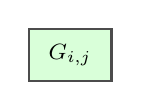
\begin{tikzpicture}
  % contract §1a `crossbar-cell`: "one weight/conductance cell in a VMM
  % array" -- the atomic, independently-copyable unit esl-crossbar-array's
  % \foreach generator instantiates nrows*ncols of.
  \node[rectangle, draw=otgray!85!black, thick, fill=weightdomain!15,
        minimum width=1.05cm, minimum height=0.66cm,
        font=\footnotesize] (cell) {$G_{i,j}$};
\end{tikzpicture}
\end{document}
